% ==============================================================================
% FICHIER : chapitre5.tex
% Description : Chapitre 5 (Sprint 2) : Gestion des Signalements et Analyse IA
% Auteurs : Dhia Fersi & Mohamed Iyed Amiri (ISET Bizerte)
% Organisme d'accueil : HRMAPS
% ==============================================================================

\chapter[Sprint 2 : Signalements et IA]{Sprint 2 : Gestion des Signalements et Analyse IA}

\section*{Introduction}
\addcontentsline{toc}{section}{Introduction}
La remontée précise, rapide et géo-localisée des anomalies urbaines est l'activité centrale des citoyens sur notre plateforme. L'objectif du Sprint 2 est de réaliser le processus complet de signalement d'un incident depuis le terrain. Pour simplifier l'expérience utilisateur et automatiser la qualification du signalement, nous intégrons un module d'Intelligence Artificielle de détection d'objets (YOLO AI) qui analyse la photo de l'anomalie pour en déduire automatiquement sa catégorie. Ce chapitre présente l'analyse de ce sprint, les diagrammes UML correspondants, et l'implémentation de la cartographie Leaflet, d'Hibernate Spatial (PostGIS) et de l'interfaçage avec l'IA.

% ------------------------------------------------------------------------------
% 1. BACKLOG SPRINT 2
% ------------------------------------------------------------------------------
\section{BACKLOG Sprint 2}
Le Backlog du Sprint 2 se concentre sur les fonctionnalités opérationnelles de signalement mobile :
\begin{itemize}
    \item \textbf{US04 -- Signalement d'incident géo-localisé (Citoyen)} : Permettre d'ouvrir la carte mobile Flutter, d'y pointer la position via GPS, de capturer une photo, d'obtenir le classement IA et d'ajouter des commentaires de départ.
    \item \textbf{US05 -- Consultation de l'état sur la carte (Citoyen)} : Permettre au citoyen de visualiser sur la carte interactive l'état actuel de l'incident (signalé, en cours, réparé).
\end{itemize}

% ------------------------------------------------------------------------------
% 2. ANALYSE ET SPÉCIFICATION DES BESOINS
% ------------------------------------------------------------------------------
\section{Analyse et spécification des besoins}

\subsection{Diagramme de cas d'utilisation}
La figure \ref{fig:uc_sprint2} illustre le cas d'utilisation détaillé de signalement d'incident.

\begin{figure}[H]
    \centering
    \framebox[\textwidth]{\vbox to 5.5cm{\vfill\hbox to \textwidth{\hss\textbf{[Figure : Diagramme de Cas d'Utilisation -- Sprint 2 (Signalement)]}\hss}\vfill}}
    \caption{Diagramme de cas d'utilisation : Sprint 2}
    \label{fig:uc_sprint2}
\end{figure}

\subsection{Description textuelle}
Voici la description textuelle du cas d'utilisation principal \textbf{« Signaler un incident »} :
\begin{itemize}
    \item \textbf{Acteur} : Citoyen.
    \item \textbf{Préconditions} : L'acteur est connecté à son compte citoyen sur l'application.
    \item \textbf{Scénario nominal} :
    \begin{enumerate}
        \item Le citoyen ouvre l'application mobile Flutter et clique sur « Signaler un incident ».
        \item L'application affiche la carte interactive Leaflet et géolocalise l'utilisateur via le GPS de son téléphone.
        \item Le citoyen capture la photo de l'anomalie directement depuis l'appareil photo du smartphone.
        \item Le client mobile envoie l'image au backend Spring Boot, qui la transfère instantanément au service YOLO AI.
        \item Le service YOLO AI renvoie la classe détectée (ex : Nid-de-poule).
        \item Le citoyen prend connaissance du choix de l'IA (qu'il peut modifier au besoin), ajoute un commentaire initial et valide le signalement.
        \item Le backend enregistre l'incident, initialise la **timeline d'évolution**, et déclenche une alerte de notification e-mail automatique à destination de l'administrateur municipal.
    \end{enumerate}
    \item \textbf{Scénarios alternatifs} : Si le microservice d'IA YOLO est indisponible, le système affiche un message d'avertissement et invite l'utilisateur à sélectionner lui-même manuellement la catégorie de l'incident dans une liste déroulante.
\end{itemize}

% ------------------------------------------------------------------------------
% 3. PRÉSENTATION ÉCRAN IHM
% ------------------------------------------------------------------------------
\section{Présentation écran IHM}
L'interface de signalement a été particulièrement optimisée pour une utilisation sur smartphone :

\begin{figure}[H]
    \centering
    \framebox[\textwidth]{\vbox to 6.5cm{\vfill\hbox to \textwidth{\hss\textbf{[Capture d'écran : Formulaire de Signalement Citoyen responsive avec carte Leaflet]}\hss}\vfill}}
    \caption{Interface de signalement mobile-first}
    \label{fig:ihm_report}
\end{figure}

% ------------------------------------------------------------------------------
% 4. DIAGRAMME DE SÉQUENCE
% ------------------------------------------------------------------------------
\section{Diagramme de séquence}
La figure \ref{fig:seq_sprint2} illustre l'interaction de signalement citoyen intégrant l'analyse d'image automatique.

\begin{figure}[H]
    \centering
    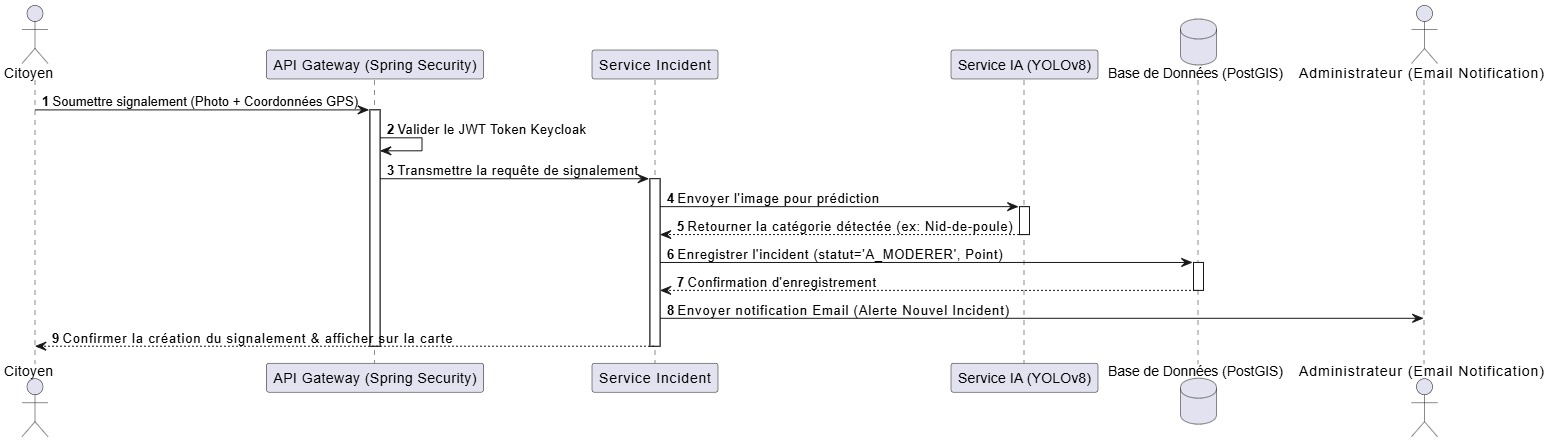
\includegraphics[width=\textwidth]{seq_signalement_yolo.jpg}
    \caption{Diagramme de séquence : Processus de signalement avec YOLO}
    \label{fig:seq_sprint2}
\end{figure}

% ------------------------------------------------------------------------------
% 5. DIAGRAMME DE CLASSES
% ------------------------------------------------------------------------------
\section{Diagramme de classes}
La figure \ref{fig:class_sprint2} montre le modèle structurel gérant l'incident, sa catégorie et sa géolocalisation.

\begin{figure}[H]
    \centering
    \framebox[\textwidth]{\vbox to 5.5cm{\vfill\hbox to \textwidth{\hss\textbf{[Figure : Diagramme de Classes -- Sprint 2 (Signalement et Données Spatiales)]}\hss}\vfill}}
    \caption{Diagramme de classes du Sprint 2}
    \label{fig:class_sprint2}
\end{figure}

% ------------------------------------------------------------------------------
% 6. RÉALISATION
% ------------------------------------------------------------------------------
\section{Réalisation}

\subsection{Intégration d'Hibernate Spatial et PostGIS}
Pour stocker et manipuler les coordonnées GPS géospatiales de manière native sous Spring Boot 3.2, nous intégrons la dépendance \texttt{hibernate-spatial}. Celle-ci étend les fonctionnalités standards de JPA/Hibernate pour supporter les types de la bibliothèque JTS (\textit{Java Topology Suite}) :

\begin{verbatim}
@Entity
@Table(name = "table_incident")
public class Incident {
    @Id
    @GeneratedValue(strategy = GenerationType.IDENTITY)
    private Long id;
    
    private String description;
    private String status;
    private String photoUrl;
    
    // Type géographique Point géré nativement par PostGIS
    private Point geom; 
    
    @ManyToOne
    @JoinColumn(name = "category_id")
    private Category category;
}
\end{verbatim}

\subsection{Intégration de la carte Leaflet}
Côté frontend mobile Flutter, nous utilisons le package \textbf{flutter\_map} (couche d'interfaçage avec Leaflet.js). L'application charge des tuiles géographiques cartographiques en mode sombre (\textit{Dark Matter}) de CartoDB, assurant une esthétique premium et reposante. Le citoyen définit l'emplacement de l'incident grâce à un marqueur tactile interactif, transmettant les coordonnées (longitude/latitude) au format standard WGS 84.

\subsection{Microservice IA YOLO}
Le backend Spring Boot communique de manière asynchrone avec un microservice écrit en Python et basé sur le framework léger FastAPI. Ce service expose une API REST de traitement d'images. À la réception de l'image chargée, le service charge un modèle de détection d'objets YOLO pré-entraîné, isole l'anomalie détectée, calcule un score de confiance (ex : $0.94$ pour un nid-de-poule), et retourne la catégorie correspondante au format JSON au backend :
\begin{verbatim}
{
  "class_name": "Nid-de-poule",
  "confidence": 0.94,
  "status": "SUCCESS"
}
\end{verbatim}

\subsection{Enchaînement des interfaces réalisées}
Sur le terrain, l'utilisateur ouvre l'application, clique sur la carte Leaflet pour localiser un incident, et appuie sur « Prendre Photo ». La photo est capturée via la caméra de l'appareil mobile, transférée au serveur, et analysée instantanément. La catégorie s'affiche sous forme de badge vert pour confirmation finale avant soumission définitive.

\section*{Conclusion}
Le Sprint 2 a permis de réaliser le cœur opérationnel de la plateforme \textit{SafeCity-Connect} pour l'expérience citoyenne. Grâce au couplage de Leaflet, Hibernate Spatial et de l'analyse automatisée par l'intelligence artificielle YOLO, la saisie d'un incident prend moins de 30 secondes pour un utilisateur sur son mobile. Le chapitre suivant détaillera le Sprint 3, qui conçoit et implémente les fonctionnalités administratives d'aide à la décision communale.
